\documentclass[notheorems]{beamer}

\usepackage{slideSFOCS}

\title{Five Days}
\author{Group 9}
\date{today}

\definecolor{do}{rgb}{0.5,0.8,.5}
\colorlet{dont}{red!65}

\newenvironment{framedd}[1][]{
	\setbeamertemplate{background}{\color{do}\rule{0.5\paperwidth}{\paperheight}\color{dont}\rule{0.5\paperwidth}{\paperheight}}
	\setslidecolor{fg=white,bg=do}
	\setbeamercolor{local structure}{fg=white}
	\begin{frame}[environment=framedd,#1]
		}{
	\end{frame}
}

\newcommand{\lcmd}[1]{{\tt \textbackslash #1}}
\pgfdeclareimage[height=0.5cm]{umji-logo}{umji-logo.png}
\logo{\pgfuseimage{umji-logo}\hspace*{0.3cm}}

\begin{document}

\maketitle

\mindtoc

\section{Who are we?}


\begin{framenl}{Who are we?}
\begin{columns}[T]
	\begin{column}<0->{.40\textwidth}
		\begin{figure}[thpb]
			\centering
			\resizebox{1\linewidth}{!}{
				
\includegraphics{figures/starcity-logo.png}
			}
		\end{figure}
	\end{column}
	\hfill
	\begin{column}<0->{.65\textwidth}
		\begin{itemize}
			\item<1-> Team members
			\begin{itemize}
		    \item Jia Zhu
            \item Xingran Shen
            \item Yang Chen
            \item Yuqi Xie
			\end{itemize}
		\end{itemize}
	\end{column}%
\end{columns}
\end{framenl}

\section{Demo}

\section{Story Background}

\begin{framenl}{Wake up}
\begin{columns}[T]
	\begin{column}<0->{0.1\textwidth}
		\begin{figure}[thpb]
			\centering
			\resizebox{1\linewidth}{!}{
				
\includegraphics{figures/day_right.png}
			}
		\end{figure}
	\end{column}
	\begin{column}<1->{0.65\textwidth}
		\begin{itemize}
			\item<1-> You, a little girl, wake up in a strange place.
			\item<2-> With a splitting headache, you found that you could only remember your name, Xiaoxiao.
		\end{itemize}
	\end{column}
	
\end{columns}	
\end{framenl}

\begin{framenl}{Encounter}
	\begin{columns}[T]
		\begin{column}<0->{0.46\textwidth}
			\begin{figure}[thpb]
				\centering
				\resizebox{1\linewidth}{!}{
					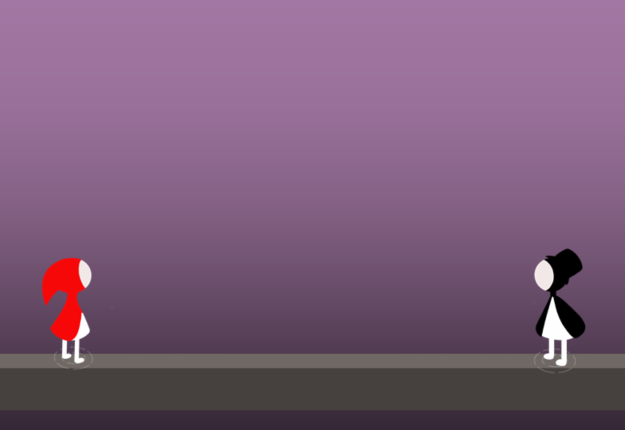
\includegraphics{figures/wakeup.png}
				}
			\end{figure}
		\end{column}
		\begin{column}<1->{0.65\textwidth}
			\begin{itemize}
				\item []
				\item <1-> Faraway, stands a guard in black
				\item <2-> Who is he? Where is this place?
				\item <3-> Go through the maze and find out the truth in the five days. 
			\end{itemize}
		\end{column}
		
	\end{columns}	
	\end{framenl}

\section{Start and prompts}

\begin{framenl}{Start}
\begin{columns}[T]
	\begin{column}<0->{.46\textwidth}
		\begin{figure}[thpb]
			\centering
			\resizebox{1\linewidth}{!}{
				
\includegraphics{figures/start.png}
			}
			
			
		\end{figure}
	\end{column}%
	\hfill%
	\begin{column}<0->{.65\textwidth}
		\begin{itemize}
			\item []
			\item [] In this game, we provide you with different laguage choice as shown: 
				\begin{itemize}
					\item English version
					\item Chinese version
				\end{itemize}
		\end{itemize}
	\end{column}%
\end{columns}
\end{framenl}


\begin{framenl}{Game prompts}
\begin{columns}[T]
\begin{column}<0->{.46\textwidth}
	\begin{figure}[thpb]
		\centering
		\resizebox{1\linewidth}{!}{
			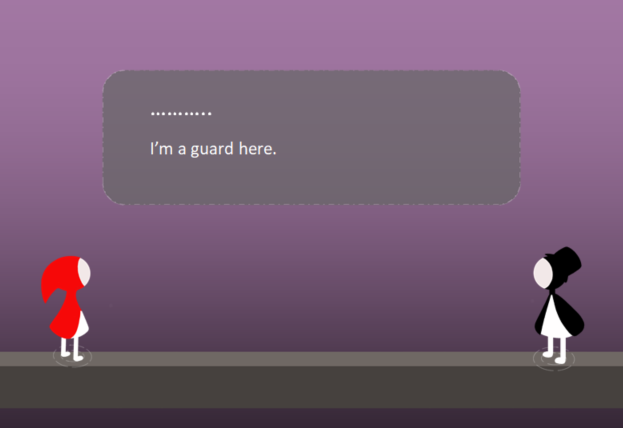
\includegraphics{figures/prompt.png}
		}
		
	\end{figure}
\end{column}%
\hfill%
\begin{column}<0->{.58\textwidth}
	\begin{itemize}
		\item<1-> Get prompts from the stranger on new things that you will encounter next during the transitional stage.
		\item<2-> Pay attetion to his word, it helps you avoid danger and go forward during the five days.
	\end{itemize}
\end{column}%
\end{columns}
\end{framenl}

% -----------------------------------------------------------------------------
\section{Game}


\begin{framenl}{Day Mode}
\begin{columns}[T] % align columns
\begin{column}<0->{.46\textwidth}
\begin{figure}[thpb]
	\centering
	\resizebox{1\linewidth}{!}{
		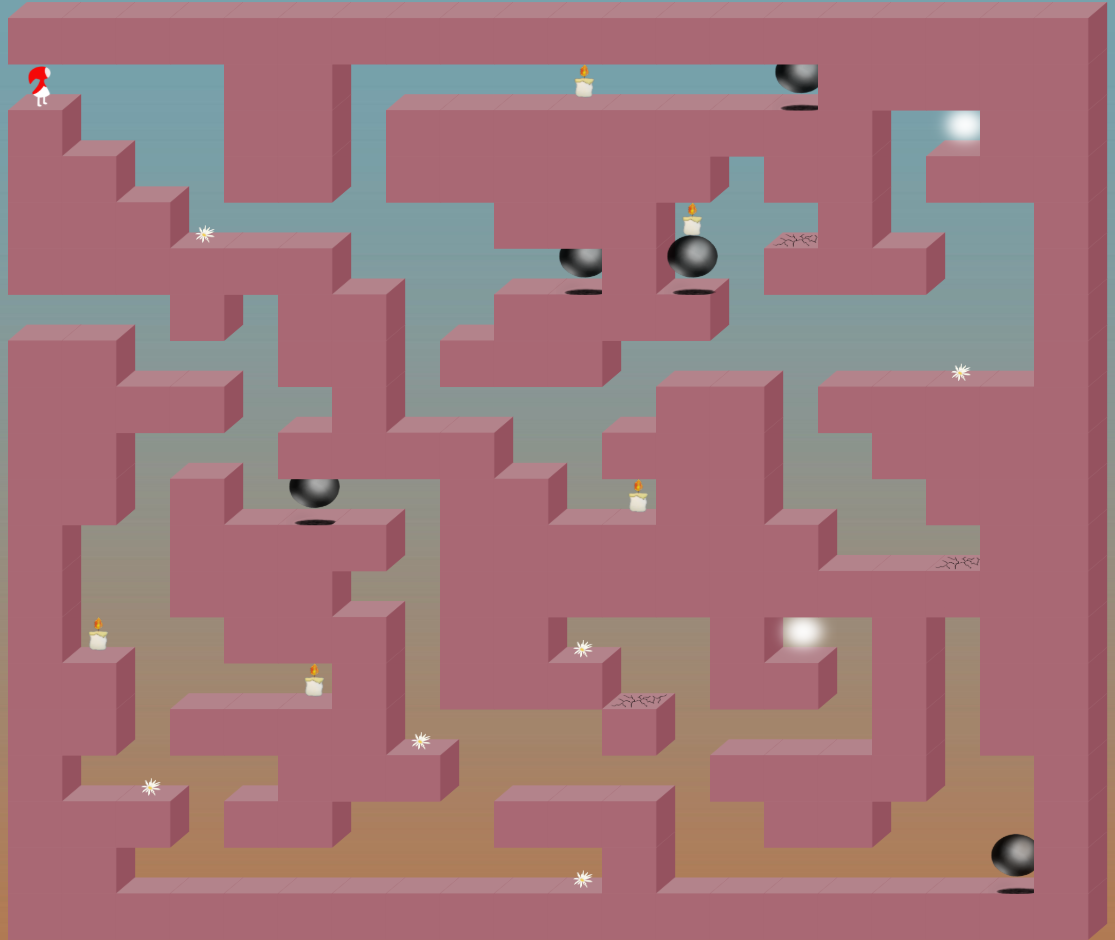
\includegraphics{figures/daymode.png}
	}
	%\includegraphics[scale=1.0]{figurefile}
	
\end{figure}
\end{column}%
\hfill%
\begin{column}<0->{.65\textwidth}
\begin{itemize}
	\item<1-> Each day, you will awake at the entrance. The whole map is shown to you.
	\item<2-> In day mode, you will encounter with these objects:
		\begin{itemize}
			\item Candles
			\item Gravity Device
			\item Cracked Floor
			\item Daisy
		\end{itemize}
\end{itemize}
\end{column}%
\end{columns}
\end{framenl}

\begin{framenl}{Candle}
\begin{columns}[T]
\begin{column}<0->{.46\textwidth}
\begin{figure}[thpb]
\centering
\resizebox{1\linewidth}{!}{
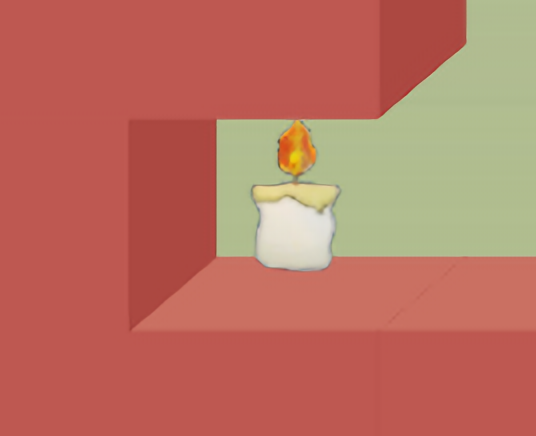
\includegraphics{figures/candle.png}
}

\end{figure}
\end{column}
\hfill
\begin{column}<0->{.65\textwidth}
\begin{itemize}
\item []
\item<1-> The amount of candles you collect during the day determines how far you can see at night
\item<2-> Start from the second day, you need to collect candle yourself.
\end{itemize}
\end{column}
\end{columns}
\end{framenl}


\begin{framenl}{Gravity Device}
\begin{columns}[T] % align columns
\begin{column}<0->{.46\textwidth}
\begin{figure}[thpb]
\centering
\resizebox{1\linewidth}{!}{
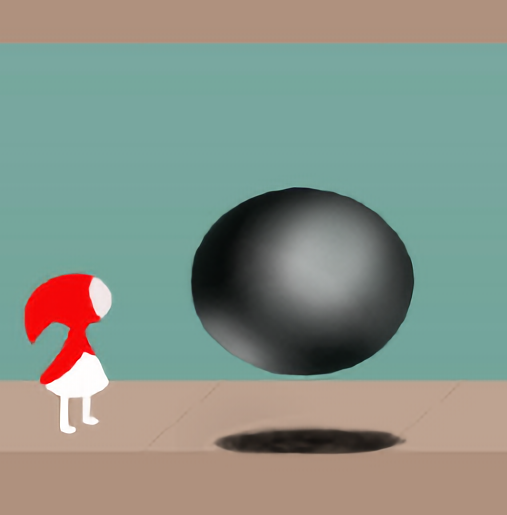
\includegraphics{figures/downwardgravity.png}
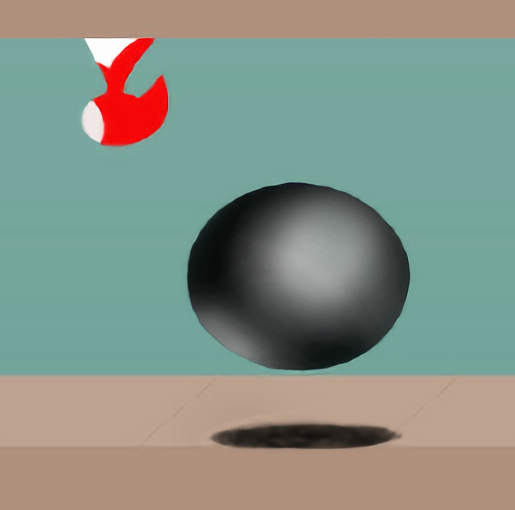
\includegraphics{figures/upwardgravity.png}
}
%\includegraphics[scale=1.0]{figurefile}
\text{Before --- After}

\end{figure}
\end{column}%
\hfill%
\begin{column}<0->{.6\textwidth}
\begin{itemize}
\item<1-> The black sphere represents the gravity device.
\item<2-> It can change the direction of the gravity between downward and upward by pressing "Space".
\item<3-> Use it wisely, it will help you a lot.
\end{itemize}
\end{column}%
\end{columns}
\end{framenl}




\begin{framenl}{Cracked Floor}
\begin{columns}[T] % align columns
\begin{column}<0->{.4\textwidth}
\begin{figure}[thpb]
\centering
\resizebox{1.3\linewidth}{!}{
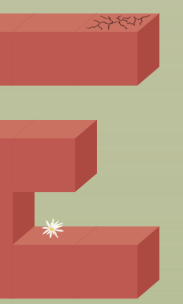
\includegraphics{figures/stationarycrackedfloor.png}
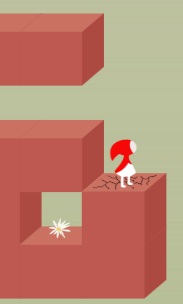
\includegraphics{figures/fallingcrackedfloor.png}
}
%\includegraphics[scale=1.0]{figurefile}
\text{The falling of cracked floor}

\end{figure}
\end{column}%
\hfill%
\begin{column}<0->{.46\textwidth}
\begin{itemize}
\item []
\item<1-> Be careful with those blocks with cracks.
\item<2-> When you step on it, it will fall in the direction of gravity.
\item<3-> Is it a trap, or something you can utilize?
\end{itemize}
\end{column}%
\end{columns}
\end{framenl}

\begin{framenl}{Daisy}
\begin{columns}[T] % align columns
\begin{column}<0->{.46\textwidth}
\begin{figure}[thpb]
\centering
\resizebox{1\linewidth}{!}{
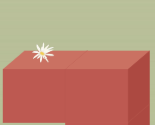
\includegraphics{figures/flower.png}
}
%\includegraphics[scale=1.0]{figurefile}

\end{figure}
\end{column}%
\hfill%
\begin{column}<0->{.65\textwidth}
\begin{itemize}
\item []
\item<1-> A beautiful white daisy, common at funerals, not wise to pick it up.
\item<2-> Who put it here? Is it related to something at night?
\end{itemize}
\end{column}%
\end{columns}
\end{framenl}


\begin{framenl}{Night Mode}
	\begin{columns}[T] % align columns
		\begin{column}<0->{.46\textwidth}
			\begin{figure}[thpb]
				\centering
					\resizebox{1\linewidth}{!}{
						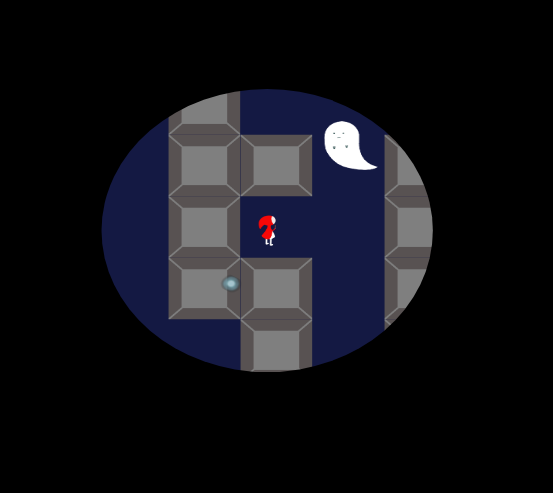
\includegraphics{figures/nightmode.png}
					}
				\end{figure}
			\end{column}%
		\hfill%
		\begin{column}<0->{.65\textwidth}
			\begin{itemize}
			\item []
			\item<1-> After you pass the day mode, press "Enter" and the map will transform to the night mode.
			\item<2-> Different from day mode, you need to pay attention to following things:
				\begin{itemize}
					\item Candle light
					\item Ghost
					\item Guide
				\end{itemize}
			\end{itemize}
		\end{column}%	
	\end{columns}
\end{framenl}

\begin{framenl}{Candle light}
	\begin{columns}[T] % align columns
		\begin{column}<0->{.46\textwidth}
			\begin{figure}[thpb]
				\centering
					\resizebox{1\linewidth}{!}{
						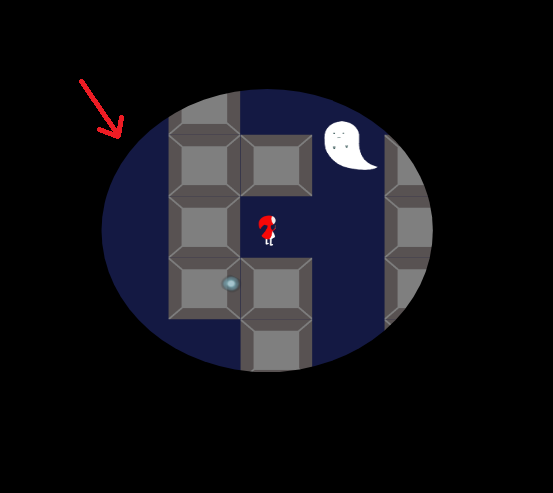
\includegraphics{figures/nightmodecandle.png}
					}
				\end{figure}
			\end{column}%
		\hfill%
		\begin{column}<0->{.65\textwidth}
			\begin{itemize}
			\item []
			\item<1-> Night falls, covered by darkness, you could only light up you candle and have limited sight.
			\item<2-> The area of the light will gradually shrink over time.
			\item<3-> Don't burn your candles out, or you will be devoured by the darkness. 
			\end{itemize}
		\end{column}%	
	\end{columns}

\end{framenl}

\begin{framenl}{Ghost}
	\begin{columns}[T] % align columns
		\begin{column}<0->{.46\textwidth}
			\begin{figure}[thpb]
				\centering
					\resizebox{1\linewidth}{!}{
						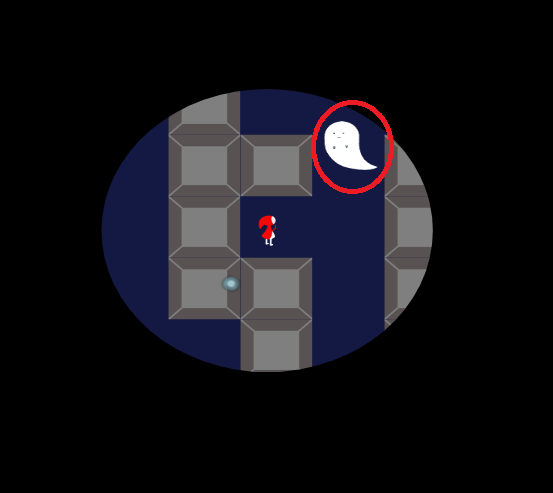
\includegraphics{figures/nightmodeghost.png}
					}
				\end{figure}
			\end{column}%
		\hfill%
		\begin{column}<0->{.65\textwidth}
			\begin{itemize}
				\item []
				\item<1-> A white ghost, caused by the spite of the dead, dangerous to approach.
				\item<2-> When it catch you, you will be fainted and sent to the entrance.
			
			\end{itemize}
		\end{column}%	
	\end{columns}

\end{framenl}


\begin{framenl}{Guide}
\begin{columns}[T] % align columns
	\begin{column}<0->{.46\textwidth}
		\begin{figure}[thpb]
			\centering
			\resizebox{1\linewidth}{!}{
			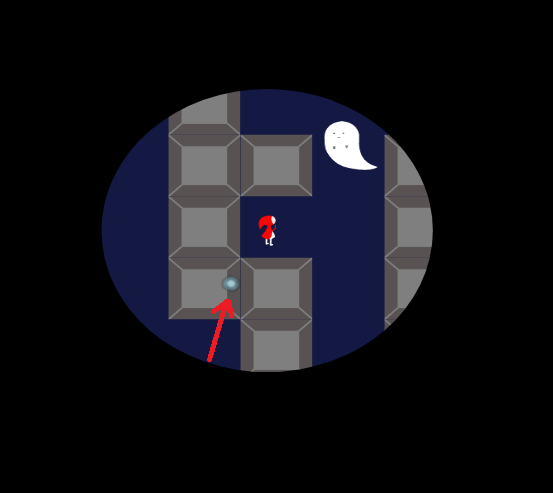
\includegraphics{figures/nightmodeguide.png}
			}
		\end{figure}
	\end{column}%
\hfill%
	\begin{column}<0->{.6\textwidth}
		\begin{itemize}
			\item []
			\item<1-> Follow the guide, it will lead you to the exit or other crucial elements in both day and night modes
		\end{itemize}
	\end{column}%
\end{columns}
\end{framenl}

\begin{framenl}{Clue}
\begin{columns}[T] % align columns
\begin{column}<0->{.46\textwidth}
\begin{figure}[thpb]
\centering
\resizebox{1\linewidth}{!}{

\includegraphics{figures/clue.png}
}
%\includegraphics[scale=1.0]{figurefile}

\end{figure}
\end{column}%
\hfill%
\begin{column}<0->{.65\textwidth}
\begin{itemize}
\item<1-> To win the game, you also need to find your memory back.
\item<2-> The white mist in the maze contains your memory and some important objects.
\item<3-> Collect them in both day and night mode.
\item <4-> The more you collect, the more chance you will have to recall.
\end{itemize}
\end{column}%
\end{columns}
\end{framenl}

\begin{framenl}{Clue List}
\begin{columns}[T] % align columns
\begin{column}<0->{.46\textwidth}
\begin{figure}[thpb]
\centering
\resizebox{1\linewidth}{!}{
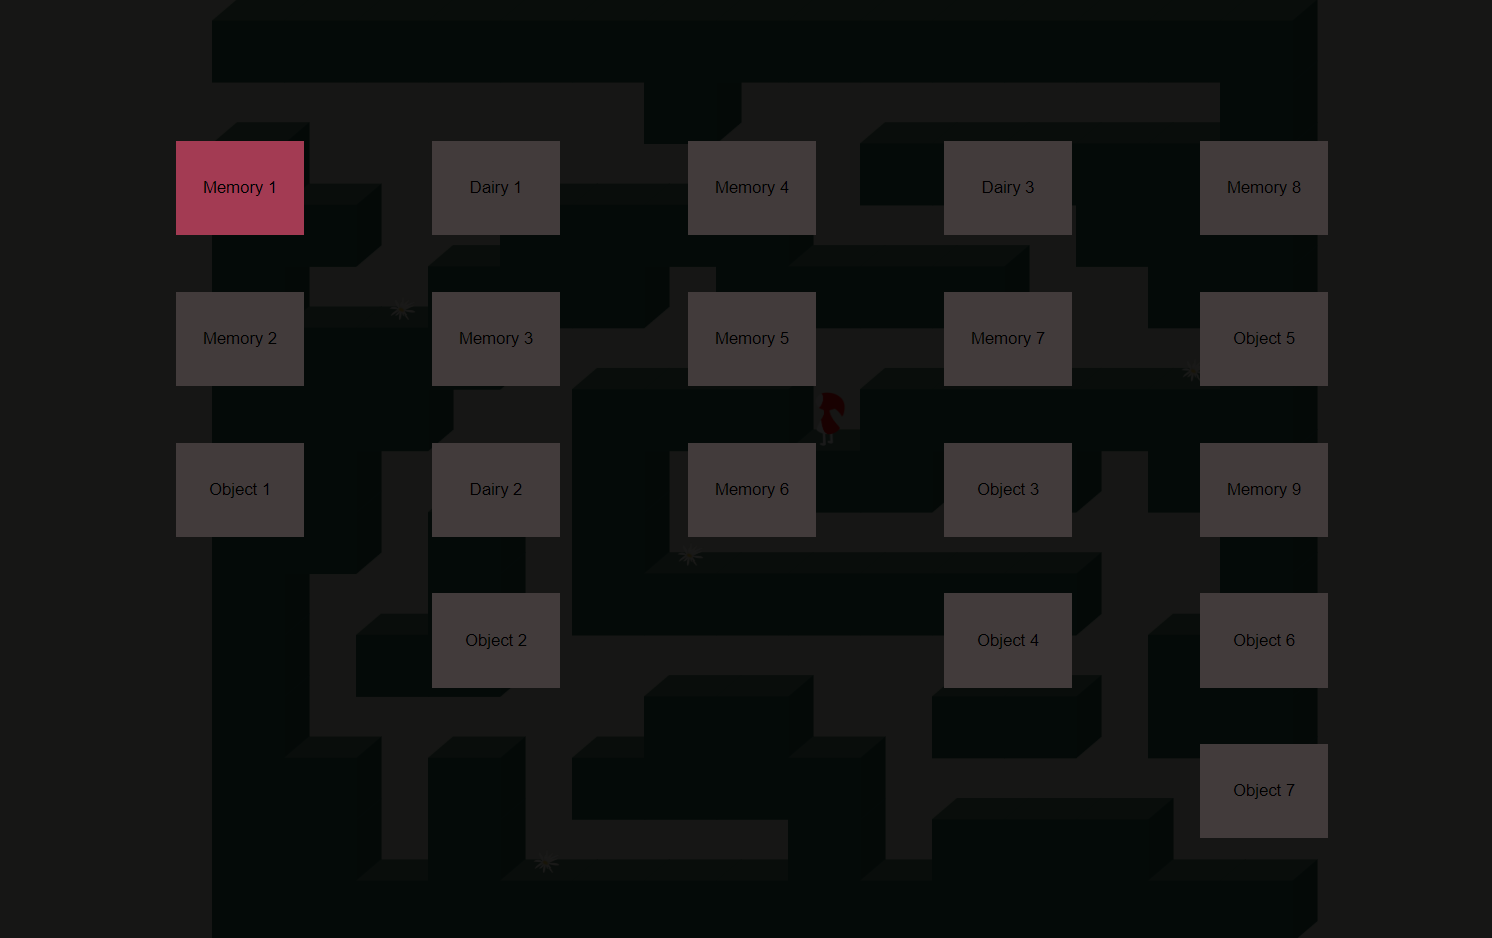
\includegraphics{figures/cluelist.png}
}
%\includegraphics[scale=1.0]{figurefile}

\end{figure}
\end{column}%
\hfill%
\begin{column}<0->{.65\textwidth}
\begin{itemize}
\item<1-> Press "c" you can open the clue list.
\item<2-> Click on the clues and you can review them. 
\item<3-> Don't worry, the game will paused when you read the clues.
\end{itemize}
\end{column}%
\end{columns}
\end{framenl}

\begin{framenl}{End Page}
\begin{columns}[T] % align columns
\begin{column}<0->{.46\textwidth}
\begin{figure}[thpb]
\centering
\resizebox{1\linewidth}{!}{
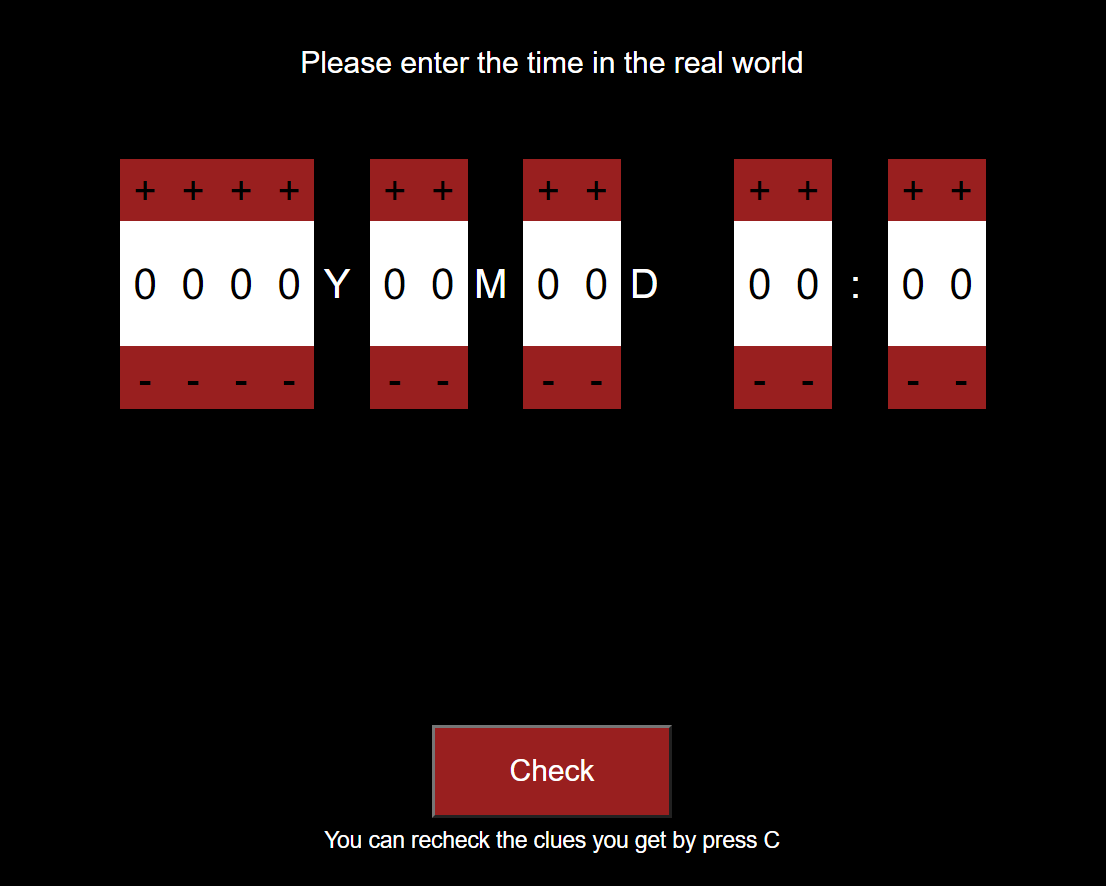
\includegraphics{figures/endpage.png}
}
%\includegraphics[scale=1.0]{figurefile}

\end{figure}
\end{column}%
\hfill%
\begin{column}<0->{.65\textwidth}
\begin{itemize}
\item []

\item<1-> Finally, you comes to here.
\item<2-> Are you ready to face the truth?
\item<3-> Use the clues, enter the date and time and get your end.
\end{itemize}
\end{column}%
\end{columns}
\end{framenl}





%\setslidecolor[fg=blue,bg=green]{fg=red,bg=orange}


\thankframe

\end{document}
